\section{eo\-Dominance\-Map$<$ Eo\-Type $>$ Class Template Reference}
\label{classeo_dominance_map}\index{eoDominanceMap@{eoDominanceMap}}
eo\-Dominance\-Map, utility class to calculate and maintain a map (std::vector$<$std::vector$<$bool$>$ $>$) of pareto dominance statistics.  


{\tt \#include $<$eo\-Dominance\-Map.h$>$}

Inheritance diagram for eo\-Dominance\-Map$<$ Eo\-Type $>$::\begin{figure}[H]
\begin{center}
\leavevmode
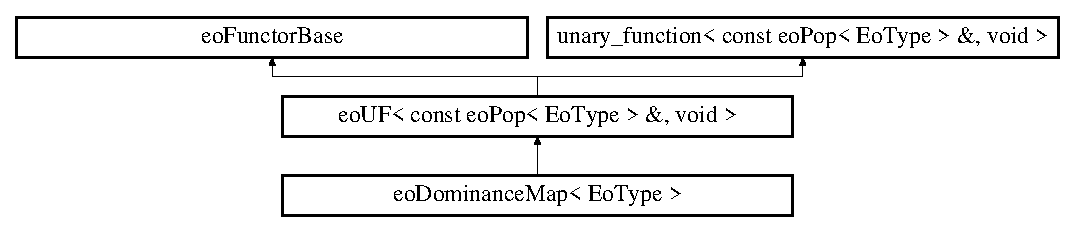
\includegraphics[height=2.67516cm]{classeo_dominance_map}
\end{center}
\end{figure}
\subsection*{Public Member Functions}
\begin{CompactItemize}
\item 
void {\bf clear} ()\label{classeo_dominance_map_a0}

\begin{CompactList}\small\item\em Clears the map. \item\end{CompactList}\item 
void {\bf operator()} (const {\bf eo\-Pop}$<$ {\bf Eo\-Type} $>$ \&\_\-pop)\label{classeo_dominance_map_a1}

\begin{CompactList}\small\item\em Update or create the dominance map. \item\end{CompactList}\item 
void {\bf remove} (unsigned i)\label{classeo_dominance_map_a2}

\begin{CompactList}\small\item\em Removes the domination info for a given individual, thus nothing dominates it and it dominates nothing. \item\end{CompactList}\item 
void {\bf setup} (const {\bf eo\-Pop}$<$ {\bf Eo\-Type} $>$ \&\_\-pop)
\begin{CompactList}\small\item\em Create domination matrix from scratch. \item\end{CompactList}\item 
std::vector$<$ double $>$ {\bf sum\_\-dominators} () const 
\begin{CompactList}\small\item\em For all elements, returns the no. \item\end{CompactList}\item 
std::vector$<$ double $>$ {\bf sum\_\-dominants} () const \label{classeo_dominance_map_a5}

\begin{CompactList}\small\item\em For all elements, returns the number of elements that the element dominates Thus: higher is better It returns a std::vector$<$double$>$ cuz that makes subsequent manipulation that much easier. \item\end{CompactList}\end{CompactItemize}
\subsection*{Private Attributes}
\begin{CompactItemize}
\item 
std::vector$<$ typename Eo\-Type::Fitness $>$ {\bf fitness}\label{classeo_dominance_map_r0}

\end{CompactItemize}


\subsection{Detailed Description}
\subsubsection*{template$<$class Eo\-Type$>$ class eo\-Dominance\-Map$<$ Eo\-Type $>$}

eo\-Dominance\-Map, utility class to calculate and maintain a map (std::vector$<$std::vector$<$bool$>$ $>$) of pareto dominance statistics. 

It is set up such that

if map[i][j] == true then i dominates j

The dominance map can be used to perform pareto ranking ({\bf eo\-Pareto\-Ranking}{\rm (p.\,\pageref{classeo_pareto_ranking})}) or non dominated sorting. For the latter, the {\bf remove()}{\rm (p.\,\pageref{classeo_dominance_map_a2})} member function might come in handy.

\begin{Desc}
\item[{\bf Todo}]make it an {\bf eo\-Stat}{\rm (p.\,\pageref{classeo_stat})}? \end{Desc}




Definition at line 47 of file eo\-Dominance\-Map.h.

\subsection{Member Function Documentation}
\index{eoDominanceMap@{eo\-Dominance\-Map}!setup@{setup}}
\index{setup@{setup}!eoDominanceMap@{eo\-Dominance\-Map}}
\subsubsection{\setlength{\rightskip}{0pt plus 5cm}template$<$class Eo\-Type$>$ void {\bf eo\-Dominance\-Map}$<$ {\bf Eo\-Type} $>$::setup (const {\bf eo\-Pop}$<$ {\bf Eo\-Type} $>$ \& {\em \_\-pop})\hspace{0.3cm}{\tt  [inline]}}\label{classeo_dominance_map_a3}


Create domination matrix from scratch. 

Complexity O(N$^\wedge$2) 

Definition at line 81 of file eo\-Dominance\-Map.h.

Referenced by eo\-Dominance\-Map$<$ EOT $>$::operator()().\index{eoDominanceMap@{eo\-Dominance\-Map}!sum_dominators@{sum\_\-dominators}}
\index{sum_dominators@{sum\_\-dominators}!eoDominanceMap@{eo\-Dominance\-Map}}
\subsubsection{\setlength{\rightskip}{0pt plus 5cm}template$<$class Eo\-Type$>$ std::vector$<$double$>$ {\bf eo\-Dominance\-Map}$<$ {\bf Eo\-Type} $>$::sum\_\-dominators () const\hspace{0.3cm}{\tt  [inline]}}\label{classeo_dominance_map_a4}


For all elements, returns the no. 

of elements that dominate the element Thus: lower is better (and 0 is the front). It returns a std::vector$<$double$>$ cuz that makes subsequent manipulation that much easier 

Definition at line 118 of file eo\-Dominance\-Map.h.

Referenced by eo\-Pareto\-Ranking$<$ EOT $>$::calculate\_\-worths().

The documentation for this class was generated from the following file:\begin{CompactItemize}
\item 
eo\-Dominance\-Map.h\end{CompactItemize}
